\documentclass{beamer}
\usepackage{tikz,amsmath,hyperref,graphicx,stackrel}
\usetikzlibrary{positioning,shadows,arrows,shapes,calc,dsp,chains}
\newcommand{\argmax}{\operatornamewithlimits{argmax}}
\newcommand{\argmin}{\operatornamewithlimits{argmin}}
\mode<presentation>{\usetheme{Frankfurt}}
\AtBeginSection[]
{
  \begin{frame}<beamer>
    \frametitle{Outline}
    \tableofcontents[currentsection,currentsubsection]
  \end{frame}
}
\title{Lecture 19: Cascaded LSI Systems}
\author{Mark Hasegawa-Johnson\\These slides are in the public domain}
\date{ECE 401: Signal and Image Analysis}
\begin{document}

% Title
\begin{frame}
  \maketitle
\end{frame}

% Title
\begin{frame}
  \tableofcontents
\end{frame}

%%%%%%%%%%%%%%%%%%%%%%%%%%%%%%%%%%%%%%%%%%%%
\section[Review]{Review: DTFT, Square Wave, Ideal Filters, and DT Processing of CT Signals}
\setcounter{subsection}{1}

\begin{frame}
  \frametitle{DTFT}

  The DTFT (discrete time Fourier transform) of any signal is
  $X(\omega)$, given by
  \begin{align*}
    X(\omega) &= \sum_{n=-\infty}^\infty x[n]e^{-j\omega n}\\
    x[n] &= \frac{1}{2\pi}\int_{-\pi}^\pi X(\omega)e^{j\omega n}d\omega
  \end{align*}
  Properties worth knowing  include:
  \begin{itemize}
  \item Time Shift: $x[n-n_0]\leftrightarrow e^{-j\omega n_0}X(\omega)$
  \item Filtering is Convolution:
    \[
    y[n]=h[n]\ast x[n]\leftrightarrow Y(\omega)=H(\omega)X(\omega)
    \]
  \end{itemize}
\end{frame}

\begin{frame}
  \frametitle{Square Wave, Rectangular Window}

  Periodic $x(t)$, with period $T_0$:
  \begin{align*}
    x(t) &= \begin{cases}1&-\frac{L}{2}\le n\le\frac{L}{2}\\
      0&\text{otherwise}
    \end{cases}\\
    X_k&= \begin{cases}
      \frac{L}{T_0} & k=0\\
      \frac{\sin(\pi kL/T_0)}{\pi k} & k\ne 0
    \end{cases}
  \end{align*}
  Aperiodic $x[n]$:
  \begin{align*}
    d_L[n] &= \begin{cases}1&-\frac{(L-1)}{2}\le n\le\frac{(L-1)}{2}\\
      0&\text{otherwise}
    \end{cases}\\
    D_L(\omega)&= \frac{\sin(\omega L/2)}{\sin(\omega/2)}
  \end{align*}
\end{frame}

\begin{frame}
  \frametitle{Discrete-Time Square Wave, Rectangular Window}

  Periodic $x[n]$, with period $T_0$:
  \begin{displaymath}
    x[n] = \begin{cases}1&-\frac{L-1}{2}< n<\frac{L-1}{2}\\
      0&\text{otherwise}
    \end{cases}~~~\leftrightarrow~~~
    X_k= \begin{cases}
      \frac{L}{T_0} & k=0\\
      \frac{\sin(\pi kL/T_0)}{T_0\sin(\pi k/T_0)} & k\ne 0
    \end{cases}
  \end{displaymath}
  \centerline{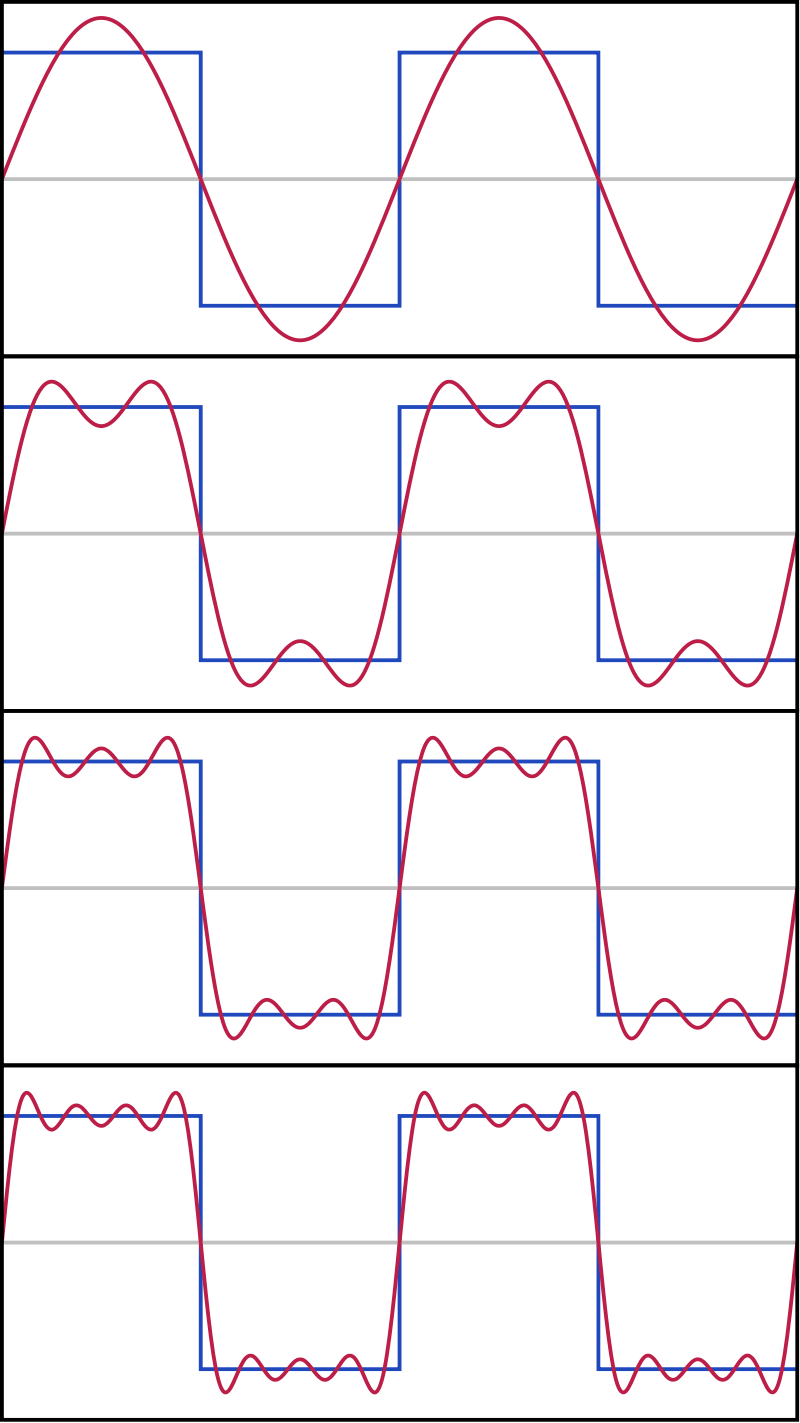
\includegraphics[height=2.5in]{exp/squarewave.png}}
\end{frame}

\begin{frame}
  \frametitle{Ideal Lowpass Filter}
  \[
  H_{LP}(\omega)
  = \begin{cases} 1& |\omega|\le\omega_c,\\
    0 & \omega_c<|\omega|\le\pi.
  \end{cases}~~~\leftrightarrow~~~
  h_{LP}[m]=\frac{\omega_c}{\pi}\mbox{sinc}(\omega_c n)
  \]
\end{frame}

\begin{frame}
  \frametitle{Review: DT Processing of CT Signals}

  A bandlimited periodic signal $x(t)$ can be sampled, filtered, then
  sinc-interpolated to create:
  \begin{align*}
    x(t)&=\sum_{k=-N}^{N}X_ke^{j2\pi kF_0t}\\
    x[n]&=\sum_{k=-N}^{N}X_ke^{jk\omega_0n},\\
    y[n]&=\sum_{k=-N}^{N}Y_ke^{jk\omega_0n},\\
    y(t)&=\sum_{k=-N}^{N}Y_ke^{j2\pi kF_0n},
  \end{align*}
  where $\omega_0=\frac{2\pi F_0}{F_s}$, and
  $N=\lfloor\frac{F_s/2}{F_0}\rfloor$, and $Y_k=H(k\omega_0)X_k$.
\end{frame}


%%%%%%%%%%%%%%%%%%%%%%%%%%%%%%%%%%%%%%%%%%%%
\section[Periodic Signals]{Response of a Filter when the  Input is Periodic}
\setcounter{subsection}{1}

\begin{frame}
  \frametitle{Response of a Filter when the Input is Periodic}

  Now we're ready to ask this question:
  \begin{block}{}
    What is the output of a filter when the  input, $x[n]$, is periodic with
    period $N_0$?
  \end{block}
\end{frame}

\begin{frame}
  \frametitle{Response of a Filter when the Input is Periodic}

  \begin{enumerate}
  \item {\bf Fourier Series:}
    If the input is periodic, then we can write  it as
    \[
    x[n] =\sum_{k=-N_0/2}^{(N_0-1)/2} X_k e^{j2\pi kn/N_0}
    \]
  \item {\bf Frequency Response:}
    If the input is $e^{j\omega n}$, then the output is
    \[
    y[n] = H(\omega)e^{j\omega n}
    \]
  \item {\bf Linearity (of convolution, and of frequency response):}
    If the input is $x_1[n]+x_2[n]$, then the output is
    \[
    y[n] = y_1[n]+y_2[n]
    \]
  \end{enumerate}
\end{frame}

\begin{frame}
  \frametitle{Response of a Filter when the Input is Periodic}

  Putting all those things together, if the input is
  \[
  x[n] =\sum_{k=-N_0/2}^{(N_0-1)/2} X_k e^{j2\pi kn/N_0}
  \]
  \ldots then the output is
  \[
  y[n] = \sum_{k=-N_0/2}^{(N_0-1)/2} X_k H(k\omega_0) e^{j2\pi kn/N_0}
  \]
  \ldots where $\omega_0=\frac{2\pi}{N_0}$ is the fundamental frequency.
\end{frame}


%%%%%%%%%%%%%%%%%%%%%%%%%%%%%%%%%%%%%%%%%%%%
\section[Pure Delay]{A Pure-Delay ``Filter''}
\setcounter{subsection}{1}

\begin{frame}
  \frametitle{A Pure-Delay ``Filter''}

  One thing we can do to a signal is to just delay it, by $n_0$ samples:
  \[
  y[n] = x[n-n_0]
  \]
  Even this very simple operation can be written as a convolution:
  \[
  y[n]=g[n]\ast x[n]
  \]
  where the ``filter,'' $g[n]$, is just
  \[
  g[n]=\delta[n-n_0] = \begin{cases}
  1 & n=n_0\\
  0 & \mbox{otherwise}
  \end{cases}
  \]
\end{frame}

\begin{frame}
  \frametitle{Frequency Response of A Pure-Delay ``Filter''}

  \[
  g[n]=\begin{cases}
  1 & n=n_0\\
  0 & \mbox{otherwise}
  \end{cases}
  \]
  The frequency response is
  \[
  G(\omega)=\sum_m g[m]e^{-j\omega m} = e^{-j\omega n_0}
  \]
  
\end{frame}

\begin{frame}
  \frametitle{Impulse Response of A Pure-Delay ``Filter''}
  Here is the impulse response of a pure-delay ``filter'' (and the magnitude and
  phase responses, which we'll talk about next).
\centerline{\includegraphics[height=2.5in]{exp/puredelay.png}}
\end{frame}

\begin{frame}
  \frametitle{Magnitude and Phase Response of A Pure-Delay ``Filter''}

  \[
  G(\omega)=\sum_m g[m]e^{-j\omega m} = e^{-j\omega n_0}
  \]
  Notice that the magnitude and phase response of this filter are
  \begin{align*}
    |G(\omega)| &= 1\\
    \angle G(\omega) &= -\omega n_0
  \end{align*}
  So, for example, if have an input of $x[n]=\cos(\omega n)$, the
  output would be
  \[
  y[n]=|G(\omega)|\cos\left(\omega n+\angle G(\omega)\right)
  = \cos\left(\omega n-\omega n_0\right)
  \]
\end{frame}


%%%%%%%%%%%%%%%%%%%%%%%%%%%%%%%%%%%%%%%%%%%%
\section[Example]{Example: Delaying a Square Wave}
\setcounter{subsection}{1}

\begin{frame}
  \frametitle{Magnitude and Phase Response of A Pure-Delay ``Filter''}
  Here are the magnitude and phase response of the pure delay filter.
\centerline{\includegraphics[height=2.5in]{exp/puredelay.png}}
\end{frame}

\begin{frame}
  \frametitle{Spectrum of a Square Wave}

  \centerline{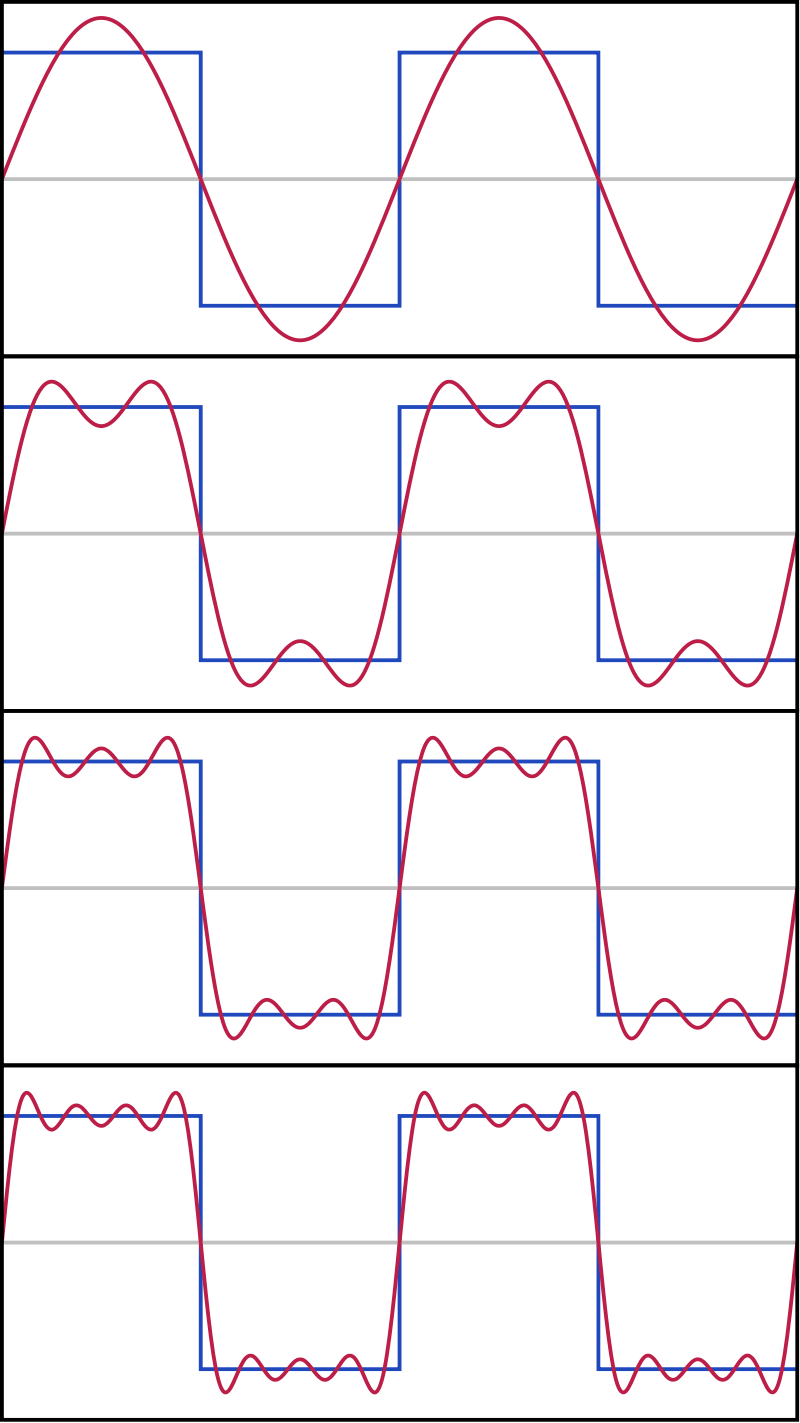
\includegraphics[height=1in]{exp/squarewave.png}}

  Here are the Fourier series coefficients of an $N_0=11$,
  $L=5$, even-symmetric square wave:
  \[
  X_k =\left.\frac{\sin(\omega L/2)}{\sin(\omega/2)}\right|_{\omega=\frac{2\pi k}{N_0}}
  =\frac{\sin(2\pi kL/N_0)}{\sin(2\pi k/N_0)}
  \]
\end{frame}

\begin{frame}
  \frametitle{Response of a Filter when the Input is Periodic}

  And here's what happens when we pass a periodic signal through a filter $g[n]$:
  \[
  x[n] =\sum_{k=-N_0/2}^{(N_0-1)/2} X_k e^{j2\pi kn/N_0}
  \]
  \[
  y[n] = \sum_{k=-N_0/2}^{(N_0-1)/2} X_k G(k\omega_0) e^{j2\pi kn/N_0}
  \]
  \ldots where $\omega_0=\frac{2\pi}{N_0}$ is the fundamental frequency.
\end{frame}

\begin{frame}
  \frametitle{Spectrum: Delayed Square Wave} And here's the result.
  This is the square wave, after being delayed by the pure-delay
  filter:
  \centerline{\includegraphics[height=2.5in]{exp/delayedsquarewave.png}}
  You can see that magnitude's unchanged, but phase is changed.
\end{frame}

\begin{frame}
  \frametitle{Spectrum of a Delayed Square Wave}

  \centerline{\includegraphics[height=1in]{exp/delayedsquarewave.png}}
  The Fourier series coefficients of a square wave, delayed by $n_0$
  samples, are
  \[
  Y_k = 
  \frac{\sin(kL\omega_0/2)}{\sin(k\omega_0/2)}e^{-jk\omega_0 n_0}
  \]
  where $\omega_0=\frac{2\pi}{N_0}$.
\end{frame}


%%%%%%%%%%%%%%%%%%%%%%%%%%%%%%%%%%%%%%%%%%%%
\section[Cascades]{Cascaded LSI Systems}
\setcounter{subsection}{1}

\begin{frame}
  \frametitle{Cascaded LSI Systems}

  What happens if we pass the input through two LSI systems, in cascade?
  \begin{center}
    \begin{tikzpicture}
      \node[dspnodeopen,dsp/label=right] (y) at (7.5,0) {$y[n]$};
      \node[dspsquare] (h) at (5,0) {${\mathcal H}$} edge[dspconn](y);
      \node[dspsquare] (g) at (2.5,0) {${\mathcal G}$} edge[dspconn](h);
      \node[dspnodeopen,dsp/label=left] (x) at (0,0) {$x[n]$} edge[dspconn](g);
    \end{tikzpicture}
  \end{center}
\end{frame}
  
\begin{frame}
  \frametitle{Cascaded filters}

  Suppose I pass the signal through filter $g[n]$, then pass it through
  another filter, $h[n]$:
  \[
  y[n]=h[n]\ast \left(g[n]\ast x[n]\right),
  \]
  we get a signal $y[n]$ whose spectrum is:
  \[
  Y(\omega)=H(\omega) G(\omega) X[k]
  \]
\end{frame}

\begin{frame}
  \frametitle{Convolution  is Commutative}

  Notice that
  \[
  Y(\omega) = H(\omega) G(\omega) X(\omega)=G(\omega)H(\omega) X(\omega)
  \]
  and therefore:
  \[
  y[n]=h[n]\ast \left(g[n]\ast x[n]\right)=g[n]\ast \left(h[n]\ast x[n]\right)
  \]
\end{frame}

\begin{frame}
  \frametitle{Convolution  is Commutative}

  Since convolution is commutative, these two circuits compute exactly the same output:
  \begin{center}
    \begin{tikzpicture}
      \node[dspnodeopen,dsp/label=right] (y) at (7.5,0) {$y[n]$};
      \node[dspsquare] (h) at (5,0) {${\mathcal H}$} edge[dspconn](y);
      \node[dspsquare] (g) at (2.5,0) {${\mathcal G}$} edge[dspconn](h);
      \node[dspnodeopen,dsp/label=left] (x) at (0,0) {$x[n]$} edge[dspconn](g);
    \end{tikzpicture}
  \end{center}
  \begin{center}
    \begin{tikzpicture}
      \node[dspnodeopen,dsp/label=right] (y) at (7.5,0) {$y[n]$};
      \node[dspsquare] (g) at (5,0) {${\mathcal G}$} edge[dspconn](y);
      \node[dspsquare] (h) at (2.5,0) {${\mathcal H}$} edge[dspconn](g);
      \node[dspnodeopen,dsp/label=left] (x) at (0,0) {$x[n]$} edge[dspconn](h);
    \end{tikzpicture}
  \end{center}
\end{frame}

\begin{frame}
  \frametitle{Quiz}

  Go to the course webpage, and try the quiz!
\end{frame}

  
\begin{frame}
  \frametitle{Example: Differenced Square Wave}

  Suppose we define $x[n]$ to be an 11-sample square wave,
  $g[n]$ to be a delay, and $h[n]$ to be a first difference:
  \[
  x[n] = \begin{cases}
    1 & -2\le n\le 2\\
    0 & 3\le n\le 8
  \end{cases}
  \]
  \[
  x[n] \stackrel{\mathcal G}{\longrightarrow} z[n] = x[n-5]
  \]
  \[
  z[n] \stackrel{\mathcal H}{\longrightarrow} y[n] = z[n]-z[n-1]
  \]
\end{frame}

\begin{frame}
  \frametitle{Delayed Square Wave}
  
  \begin{center}
    \begin{tikzpicture}
      \node[dspnodeopen,dsp/label=right] (y) at (5,0) {$y[n]$};
      \node[dspsquare] (g) at (2.5,0) {${\mathcal G}$} edge[dspconn](y);
      \node[dspnodeopen,dsp/label=left] (x) at (0,0) {$x[n]$} edge[dspconn](g);
    \end{tikzpicture}
  \end{center}
  Here's what we get if we just {\bf delay} the square wave:
  \centerline{\includegraphics[height=2in]{exp/delayedsquarewave.png}}
\end{frame}

\begin{frame}
  \frametitle{Differenced Square Wave}
  
  \begin{center}
    \begin{tikzpicture}
      \node[dspnodeopen,dsp/label=right] (y) at (5,0) {$y[n]$};
      \node[dspsquare] (g) at (2.5,0) {${\mathcal H}$} edge[dspconn](y);
      \node[dspnodeopen,dsp/label=left] (x) at (0,0) {$x[n]$} edge[dspconn](g);
    \end{tikzpicture}
  \end{center}
  Here's what we get if we just {\bf difference} the square wave:
  \centerline{\includegraphics[height=2in]{exp/differenced_squarewave.png}}
\end{frame}

\begin{frame}
  \frametitle{Example: Differenced Delayed Square Wave}

  \begin{center}
    \begin{tikzpicture}
      \node[dspnodeopen,dsp/label=right] (y) at (7.5,0) {$y[n]$};
      \node[dspsquare] (h) at (5,0) {${\mathcal H}$} edge[dspconn](y);
      \node[dspsquare] (g) at (2.5,0) {${\mathcal G}$} edge[dspconn](h);
      \node[dspnodeopen,dsp/label=left] (x) at (0,0) {$x[n]$} edge[dspconn](g);
    \end{tikzpicture}
  \end{center}
  Here's what we get if we {\bf delay} and then {\bf difference} the square wave:
  \centerline{\includegraphics[height=2.5in]{exp/differenced_delayed_squarewave.png}}
\end{frame}

\begin{frame}
  \frametitle{Example: Delayed Differenced Square Wave}

  \begin{center}
    \begin{tikzpicture}
      \node[dspnodeopen,dsp/label=right] (y) at (7.5,0) {$y[n]$};
      \node[dspsquare] (h) at (5,0) {${\mathcal G}$} edge[dspconn](y);
      \node[dspsquare] (g) at (2.5,0) {${\mathcal H}$} edge[dspconn](h);
      \node[dspnodeopen,dsp/label=left] (x) at (0,0) {$x[n]$} edge[dspconn](g);
    \end{tikzpicture}
  \end{center}
  Here's what we get if we {\bf difference} and then {\bf delay} the square wave
  (hint: it's exactly the same as the previous slide!!)  
  \centerline{\includegraphics[height=2.5in]{exp/delayed_differenced_squarewave.png}}
\end{frame}

\begin{frame}
  \frametitle{Magnitude and Phase of Cascaded Frequency Responses}

  In general, when you cascade two LSI systems, the magnitudes multiply:
  \[
  |Y_k|=|H(\omega)||G(\omega)||X_k|,
  \]
  but the phases add:
  \[
  \angle Y_k = \angle H(\omega)+\angle G(\omega)+\angle X_k
  \]
  That's because:
  \[
  H(\omega)G(\omega)=|H(\omega)|e^{j\angle H(\omega)}|G(\omega)|e^{j\angle G(\omega)}
  =|H(\omega)||G(\omega)| e^{j\left(\angle H(\omega)+\angle G(\omega)\right)}
  \]
\end{frame}


%%%%%%%%%%%%%%%%%%%%%%%%%%%%%%%%%%%%%%%%%%%%
\section[Summary]{Summary}
\setcounter{subsection}{1}

\begin{frame}
  \frametitle{Summary}
  \begin{itemize}
  \item {\bf Periodic inputs:}
    If the input of an LSI system is periodic,
    \[
    x[n] =\sum_{k=-N_0/2}^{(N_0-1)/2} X_k e^{j2\pi kn/N_0}
    \]
    \ldots then the output is
    \[
    y[n] = \sum_{k=-N_0/2}^{(N_0-1)/2} X_k H(k\omega_0) e^{j2\pi kn/N_0}
    \]
  \item {\bf Cascaded LTI Systems} convolve their impulse responses, equivalently, they
    multiply their frequency responses:
    \[
    y[n]=h[n]\ast g[n]\ast x[n],~~~Y_k=H(k\omega_0)G(k\omega_0)X_k
    \]
  \end{itemize}
\end{frame}

\end{document}
